\documentclass[lettersize,journal]{IEEEtran}
\usepackage{amsmath,amsfonts}
\usepackage{algorithm}
\usepackage{algorithmic}
\usepackage{array}
\usepackage[caption=false,font=normalsize,labelfont=sf,textfont=sf]{subfig}
\usepackage{textcomp}
\usepackage{stfloats}
\usepackage{url}
\usepackage{verbatim}
\usepackage{graphicx}
\usepackage{balance}
\usepackage{amssymb}
\usepackage{bm}

\hyphenation{op-tical net-works semi-conduc-tor IEEE-Xplore}

\begin{document}

\title{Joint Passage Direction and Entrance-Rate Optimization for Large-Scale Crowd Control in Open Pedestrian Zones: A Bellman Conservation Law Approach}

\author{Author Name
\thanks{The author is with the Department, Institution, City, Country (e-mail: email@address).}}

% \markboth{Journal Name,~Vol.~XX, No.~X, Month~2026}%
% {Author: Channel Optimization for Crowd Management}

\maketitle

\begin{abstract}
Open scenic areas and major event venues often face systematic stampede risks caused by highly concentrated pedestrian flows, while existing large-scale crowd control methods largely rely on empirical rules and post-event reviews, making active prevention and quantitative evaluation difficult.
In such scenarios, the principal operational controls are to set passage directions, including one-way, two-way, and closed states, and to regulate time-varying entrance release intensities; however, the coupled effects of these two types of controls on global pedestrian flow still lack quantitative modeling and optimization tools.
To address this problem, this paper proposes a macroscopic crowd dynamics modeling and control-measure optimization method for fine-grained large-scale crowd management.
The model is built upon the Hughes continuum framework.
To represent operational rules in a continuum setting, local admissible direction sets are introduced to characterize discrete control states such as one-way movement, two-way movement, and channel closure, while anisotropic mobility tensors describe the geometric guidance exerted by channel layouts on pedestrian flow.
On this basis, internal channel entrance flow-rate control is further introduced, enabling a control strategy to jointly specify travel directions and time-varying release intensities.
To solve the resulting mixed-variable optimization problem composed of discrete direction configurations and continuous release intensities, this paper designs a Hierarchical Constrained Mixed-variable Black-box Optimization (HCMBO) algorithm for searching optimal crowd control strategies.
Experiments on a simplified scenic-platform scenario show that the proposed macroscopic model can capture the complex interactions among multi-stage behavior, channel geometric guidance, and direction constraints.
Under a weighted composite of efficiency, safety, load-balance, waiting, and smoothness terms, repeated experiments show that HCMBO achieves the lowest mean objective value.
It reduces the objective by approximately 3.9\% compared with the second-best TPE-style mixed Bayesian optimization method, and also outperforms random search, pure simulated annealing, differential evolution, and other baseline methods.
The proposed method provides a quantitative and interpretable decision-support tool for crowd routing and entrance flow control in open public spaces.
\end{abstract}

\begin{IEEEkeywords}
Crowd dynamics modeling, crowd flow control, mixed-variable black-box optimization.
\end{IEEEkeywords}

\section{Introduction}
\label{sec:introduction}

\IEEEPARstart{L}{arge-scale} crowd gathering poses risks not only to individual safety but also to public order, as localized congestion can escalate into stampede incidents. Effective crowd management is therefore a critical component of urban public-safety governance \cite{RN2147,RN1998}.
High-density pedestrian activities, such as holiday tourism, public events, and major sports gatherings, are becoming increasingly frequent.
As a result, core urban areas must accommodate pedestrian demands far exceeding daily levels within short time windows, which poses major challenges for on-site organization, risk early warning, and emergency dispatch \cite{RN2154,RN1193,RN673}.
Against this backdrop, scientific modeling, numerical simulation, and optimization of crowd-control strategies have become critical research problems for social safety and urban governance \cite{RN1226,RN2059}.
Such methods aim to improve the efficiency of large-scale event organization while reducing local congestion risks.

Crowds in large-scale events constitute typical complex systems.
Numerous individuals with heterogeneous desired speeds, destinations, and route preferences interact through multi-scale, nonlinear mechanisms in confined spaces, generating spatiotemporal patterns at the collective level \cite{RN1193,RN1100}.
Macroscopically, these patterns appear as destination-oriented flow, passage convergence, bottleneck queuing, and directional responses to control regulations \cite{RN2056,RN2102}.
Microscopically, individuals are influenced by surrounding density, visible paths, obstacles, and guidance facilities \cite{RN2174}.
For open scenic areas, crowd behavior additionally exhibits pronounced phase dependence: visitors may first move toward a sightseeing platform, then tour along the main viewing direction, and subsequently choose different exit passages based on preferences \cite{RN2302}.
These characteristics of multi-stage, multi-route coexistence with shared congestion mean that traditional static capacity analysis or single shortest-path models cannot adequately support refined management decisions.

Among various urban crowd gathering scenarios, open scenic areas, waterfront sightseeing platforms, and historic commercial districts are highly representative.
Unlike enclosed venues such as stadiums and subway stations with well-defined boundaries \cite{RN761,RN2194}, such areas consist of open spaces, main tourist corridors, multiple lateral connecting passages, and return flow lines.
In these settings, visitors typically undergo a continuous behavioral chain of ``entry--touring along the main corridor--choosing passages to leave--returning'' \cite{RN2301}.
Their movement is therefore governed jointly by spatial geometry, control regulations, and historical behavioral preferences \cite{RN2303}.
Taking the Shanghai Nanjing East Road--Bund area as a concrete example, visitors approach the Bund from Nanjing East Road, ascend to the Bund sightseeing platform via multiple stepped passages, tour along the waterfront, then exit through several southern passages and return along lower streets.
This scenario can be abstracted as the typical ``Bund sightseeing platform--multi-stepped passage'' crowd flow scenario.
In such scenarios, management difficulties appear in three aspects.
First, multiple passages simultaneously serve entry, exit, and diversion functions, so local direction settings can alter the overall flow organization.
Second, behavioral transitions between the main tourist corridor and lateral passages make single origin--destination models insufficient.
Third, local congestion and global route choice form feedback loops, where control changes in one passage may redistribute loads in adjacent areas.

\begin{figure*}[!t]
\centering
\subfloat[]{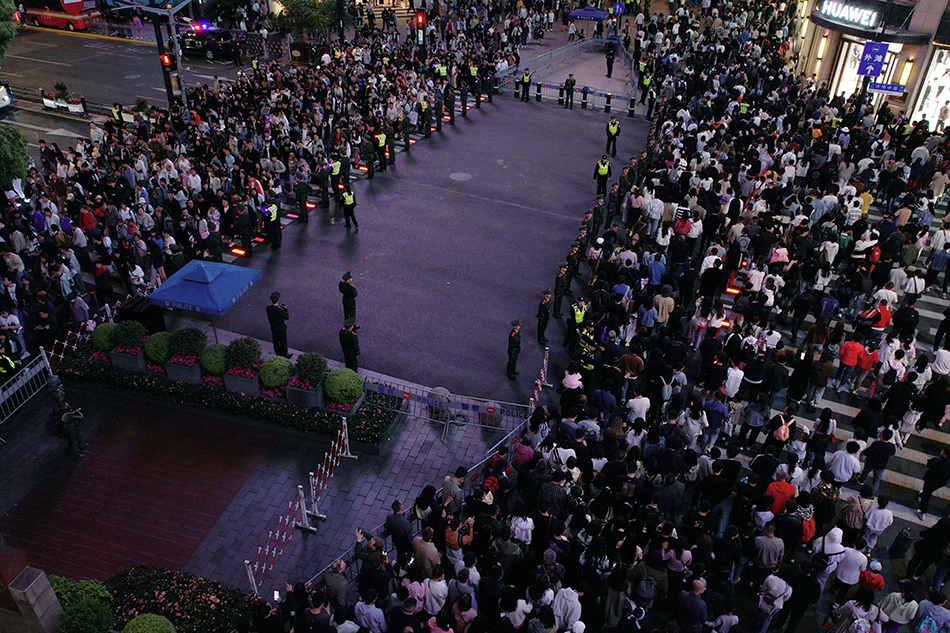
\includegraphics[width=0.47\textwidth]{../images/外滩场景/63988092.jpeg}
\label{fig:bund_scene_crowd}}
\hfill
\subfloat[]{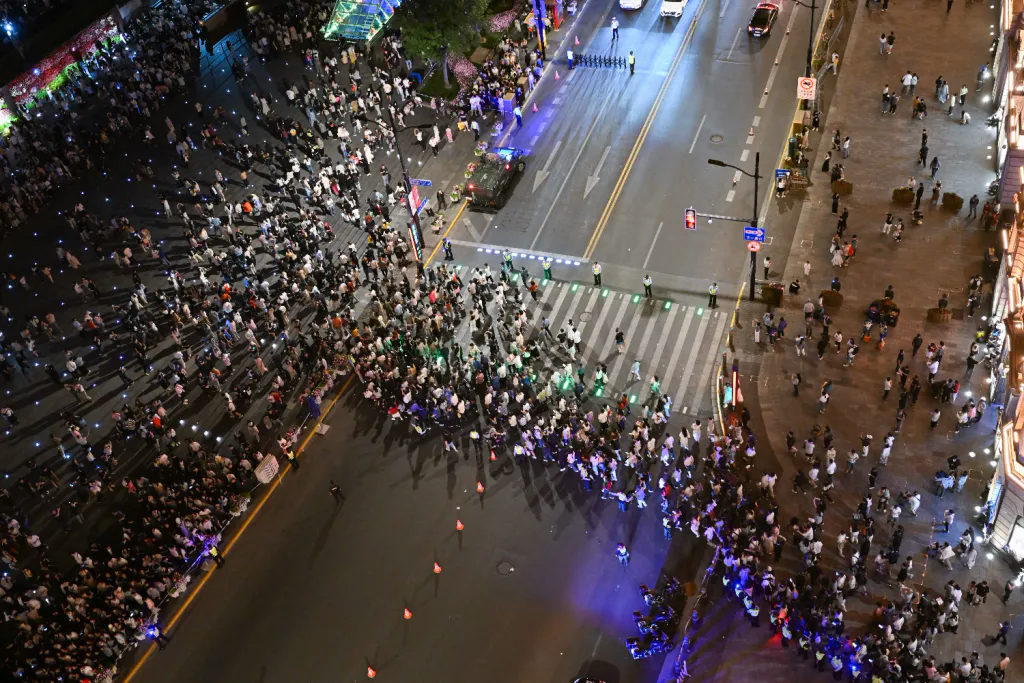
\includegraphics[width=0.47\textwidth]{../images/外滩场景/入口容量控制.png}
\label{fig:bund_scene_capacity}}
\caption{Field-control context of the Shanghai Nanjing East Road--Bund area. (a) Large-scale holiday crowd under one-way passage organization; image source: \cite{qq2024huangpu_security}. (b) Entrance-capacity control at a main visitor inflow location; image source: \cite{chinanews2019bund_flow_guidance}.}
\label{fig:bund_scene}
\end{figure*}

Existing large-scale event security management practices typically integrate system dynamics, system coupling, and system safety theory, combined with high-risk zone delineation and historical crowd behavior patterns, to formulate a series of control measures \cite{RN2176,RN1663}.
These measures include deploying security personnel at critical locations, erecting temporary barriers for isolation and diversion, implementing one-way organization on key passages, and applying batch release in core areas \cite{RN2181,RN1978}.
For instance, during major holidays, the Shanghai Bund area adopts batch release, passage direction regulation, south-entry north-exit routing, and reduction of head-on conflicts \cite{RN2129}; similarly, Nanluoguxiang main street in Beijing implements one-way passage measures (south entry, north exit) during peak periods \cite{RN2130}, consistent in control mechanism with the Shanghai Bund approach.

However, current management practices in urban high-pedestrian-flow areas remain heavily reliant on manual experience and static contingency plans, and still fall short in scientific evaluation and fine-grained optimization \cite{RN1662}.
First, many control schemes are derived from historical experience and lack a quantitative characterization of how passage direction settings, entrance release capacities, and phase-dependent behavioral preferences shape crowd dynamics.
Second, existing methods tend to rely on single-point statistics or local density monitoring, which makes it difficult to capture the dynamic coupling among ``passage direction rules--entrance flow control--local optimal directions--collective density evolution--exit load distribution'' \cite{RN2124}.
Third, in open scenic areas with multiple entrances, passages, and stages, neglecting visitor route preferences and phase-transition behaviors can lead to misjudgment of passage loads and high-risk locations.
Fourth, many simulation- and optimization-based methods treat the crowd model as a black-box evaluator and fail to exploit the structural information embedded in passage geometry, one-way rules, internal entrance capacities, and multi-route subpopulations \cite{RN2146}, which renders control-strategy search inefficient \cite{RN2122}.
Finally, although evacuation-model verification and validation studies have emphasized component-level testing and emergent-behavior validation \cite{ronchi2016vv_evacuation_models}, existing crowd-control optimization studies still lack an evaluation structure that explicitly separates mechanism diagnostics from strategy-level management objectives.

To address the above issues, this paper proposes a macroscopic crowd modeling and control optimization framework for the ``Bund sightseeing platform--multi-stepped passage'' open scenic area scenario.
The framework connects multi-stage pedestrian movement, passage direction management, geometric guidance, and entrance release control in a unified simulation-and-optimization workflow.
It aims to provide a quantitative basis for comparing candidate crowd-control strategies under limited simulation budgets, rather than relying only on empirical rules or post-event assessment.

The main contributions of this paper are as follows.

\begin{enumerate}
\item We formulate a multi-stage, multi-route macroscopic model for the open scenic-area class represented by the Bund sightseeing platform and its connected passages. Unlike single-origin--destination or single-potential Hughes-type formulations, the model lets entry, sightseeing, exit, return movement, and route redistribution arise through shared congestion.

\item We develop a Bellman--conservation-law operator that combines hard direction rules, anisotropic mobility guidance, and internal entrance-rate metering. This unified macroscopic operator represents one-way, two-way, and closed channels, channel pre-alignment, open-but-metered entrances, and upstream waiting under mass-consistent dynamics.

\item We establish an evaluation protocol that separates behavioral-mechanism diagnostics from strategy-level management objectives. The protocol first checks whether direction constraints and geometric guidance behave as intended, and then compares policies by efficiency, high-density exposure, load balance, entrance waiting, and control smoothness.

\item We design a hierarchical constrained mixed-variable black-box optimization framework (HCMBO) for joint direction and entrance-rate control. By exploiting the direction--capacity structure and applying unified high-fidelity rechecking, HCMBO achieves the best mean objective among representative mixed-variable baselines under the tested budget.
\end{enumerate}

\section{Related Work}
\label{sec:related}

\subsection{Massive Crowd Management and Control}

Crowd management in urban centers has been extensively studied from control-theoretic and optimization perspectives, aiming to enhance safety and efficiency through boundary regulation, facility layout, and intelligent decision-making \cite{RN2000,RN2193}.

In control-theoretic approaches, Zhong et al. \cite{RN279} designed boundary control strategies for urban traffic flow networks to ensure convergence to uncongested states under disturbances, with stability analysis based on Lyapunov methods \cite{RN1196}.
For one-dimensional crowd dynamics, Wadoo and Kachroo \cite{RN280} employed advection and diffusion control to prevent blocking and shock waves during evacuation.
Addressing multi-directional disturbance propagation, Qin \cite{RN277} proposed a unit sliding mode controller based on integral barrier Lyapunov functions to ensure boundedness of internal state variables, demonstrating strong disturbance rejection capabilities.
For heterogeneous corridor regulation, Zhu et al. \cite{RN286} combined policy learning with neural networks to learn optimal feedback controllers that adjust inflow rates and free-flow speeds, achieving balanced density distribution and reduced congestion.

Physical infrastructure regulation has also proven effective.
Studies have shown that strategically placed obstacles can significantly improve outflow, velocity, and local density in merging areas \cite{RN1662,RN2145}.
Yang et al. \cite{RN2118,RN2120} employed Model Predictive Control (MPC) to optimize barrier lengths at subway bottlenecks, later extending control variables to entrance limiters, gates, and escalator directions for dynamic, real-time crowd regulation.
For evacuation guidance, Carmona and Paricio-Garcia \cite{RN2119} proposed dynamic exit-choice recommendations using multinomial Logit models.
However, their approach relies on discrete speed instructions (e.g., ``stop,'' ``walk,'' ``run'') transmitted via electronic wristbands \cite{RN2196}, which poses implementation challenges in open urban scenarios.

Recently, intelligent optimization and deep reinforcement learning have emerged as promising alternatives.
Liao et al. \cite{RN2121} formulated fence layout as a subset selection problem, while subsequent work \cite{RN2122} proposed a dynamic crowd inflow control system using LSTM networks to capture temporal features and Proximal Policy Optimization (PPO) \cite{RN2189} for real-time entrance flow regulation.
Differential Evolution (DE) \cite{RN2190} has also been applied to optimize guardrail layouts and flow guidance in real-world scenarios such as Chengdu East Railway Station, using average travel time and crowd pressure as multi-objective criteria \cite{RN2123}.

\subsection{Macroscopic Crowd Modeling}

Macroscopic crowd models treat pedestrian flows as continuous media, offering computational efficiency and analytical tractability compared to microscopic approaches.
Henderson \cite{RN282} first applied fluid dynamics to pedestrian traffic in the early 1970s, comparing crowd motion to the behavior of gas or fluid particles.

Hughes \cite{hughes2003} pioneered the first-order continuum theory for pedestrian flow, introducing the classical model in which pedestrian walking speed is governed by local density through a fundamental diagram, while movement direction follows the steepest-descent path of a potential function representing the remaining travel time to exits.
This framework elegantly captures the interplay between congestion and route choice.
Ling et al. \cite{RN2078} subsequently generalized the Hughes formulation and developed an efficient numerical solution combining a weighted essentially non-oscillatory (WENO) scheme for the conservation law with a fast sweeping method for the eikonal equation.

Several extensions have enriched the descriptive capability of macroscopic models.
Nonlocal flux models were proposed by Colombo et al. \cite{RN2097}, replacing pointwise density with a neighborhood-averaged quantity in the velocity function to account for anticipatory behavior.
This direction was further extended to incorporate anisotropic perception fields and boundary effects from walls and obstacles, with high-resolution numerical schemes and well-posedness results suitable for realistic architectural configurations \cite{RN2080}.
To enforce the hard incompressibility constraint---that pedestrian density cannot exceed a physically admissible maximum---Maury et al. \cite{RN2099} introduced the projection model, which formulates the actual velocity as a least-squares projection of the desired velocity onto the set of feasible (non-overlapping) configurations.
This framework was later recast as a Wasserstein gradient flow with density constraints \cite{RN2081}, using the Jordan--Kinderlehrer--Otto (JKO) scheme \cite{RN2188} to discretize the motion while guaranteeing that density respects an upper bound, making it well-suited for high-density congestion scenarios.

To overcome non-physical behaviors such as supersonic information propagation that may arise in first-order models, Aw and Rascle \cite{RN2103} introduced a second-order model based on a generalized momentum conservation law that preserves anisotropy.
The Aw--Rascle (AR) framework was subsequently adapted to pedestrian flows \cite{RN2104}, where the congestion pressure term successfully reproduces characteristic phenomena including stop-and-go waves and spontaneous lane formation.

Beyond the classical Hughes-type framework, extensions have incorporated control and guidance mechanisms relevant to crowd management.
Anisotropic formulations using mobility tensors have been developed to represent channel geometries and directional preferences \cite{cristiani2016,priuli2015control}, allowing for continuous geometric guidance without explicit prohibition.
Constrained Hamilton-Jacobi-Bellman (HJB) formulations have been employed to model strict directional constraints such as one-way corridors, with the Bellman optimality principle providing a natural framework for unifying anisotropic geometric guidance with discrete directional constraints.

Despite these advances, existing approaches often treat control parameters as fixed or manually tuned.
The joint optimization of discrete channel direction configurations and internal entrance capacity profiles remains underexplored, particularly for large-scale urban pedestrian zones with multiple behavioral stages and heterogeneous route choices.

\section{Methodology}
\label{sec:model}

\subsection{Problem Definition and Overall Framework}

We address a multi-channel crowd management problem in open scenic areas.
The proposed method combines a Bellman--conservation-law crowd dynamics model \cite{hughes2003,RN2078} with a joint direction-capacity control formulation.
The controllable management variable is defined as
\begin{equation}
z=(s,q)\in\mathcal Z,
\label{eq:control_variable}
\end{equation}
where $s$ denotes the discrete direction states of the channels, and $q$ denotes the time-varying internal entrance capacity profile.
The behavioral preference parameter $\hat p$ and the geometric guidance parameter $\eta_0$ are treated as fixed model inputs.
For a given control variable $z$, the lower-level simulator returns density fields, velocity fields, entrance waiting, and realized channel throughputs.
The upper-level optimizer then evaluates efficiency, safety, load balance, waiting, and smoothness metrics, and searches for a better control policy under a limited simulation budget.
The overall method framework is shown in Fig.~\ref{fig:method_framework}.

\begin{figure*}[!t]
\centering

\includegraphics[width=\textwidth]{../images/framework/method_framework_tikz.pdf}
\caption{Method framework for joint direction and entrance-rate optimization. Fixed scenario inputs, behavioral preferences, and geometric guidance parameters define the lower-level Bellman--conservation-law crowd simulator. The controllable direction configuration and entrance-rate profile are jointly evaluated by efficiency, safety, load-balance, waiting, and smoothness objectives, and are updated by the upper-level HCMBO optimizer.}
\label{fig:method_framework}
\end{figure*}

The key modeling assumption is that direction rules and entrance capacities should be optimized jointly.
The direction configuration $s$ changes the local feasible direction set, whereas the entrance capacity $q$ changes the realized admitted flux at channel entrances.
These two controls jointly affect channel loading, local high-density exposure, and upstream waiting.
Therefore, we formulate crowd management as a mixed-variable simulation-based optimization problem rather than as two independent subproblems, consistent with recent simulation-based passenger-flow and entrance-control studies \cite{RN2122,jiang2018coordinated_inflow,liu2021queuing_network_flow_control}.

\subsection{Bellman--Conservation-Law Crowd Dynamics}

\subsubsection{Conservation Law and Speed Function}

We consider a bounded two-dimensional domain $\Omega \subset \mathbb{R}^2$ representing the pedestrian walking area.
Let $\Omega_w\subset\Omega$ denote the walkable region, $\rho(x,t)$ the total crowd density, and $\mathbf v(x,t)$ the local mean velocity.
Mass conservation is governed by
\begin{equation}
\frac{\partial \rho}{\partial t} + \nabla \cdot (\rho \mathbf{v}) = 0.
\label{eq:continuity}
\end{equation}

The speed magnitude is determined by local congestion.
We adopt the Greenshields-type speed function
\begin{equation}
f(\rho) = v_{\max}\left(1 - \frac{\rho}{\rho_{\max}}\right)_+,
\label{eq:greenshields}
\end{equation}
where $v_{\max}$ is the free-flow speed, $\rho_{\max}$ is the maximum admissible density, and $(\cdot)_+$ denotes nonnegative truncation.
This function captures the feedback that pedestrians move close to free-flow speed in low-density regions and slow down as density approaches congestion.

The classical Hughes model assumes that all movement directions are feasible and isotropic \cite{hughes2003}.
This assumption is insufficient for crowd management scenarios involving one-way rules, temporary closures, entrance metering, and channel-axis alignment.
The following subsections introduce admissible direction sets, anisotropic mobility tensors, and internal entrance capacity control into the Bellman--conservation-law framework.

\subsubsection{Multi-Stage Multi-Route Density Decomposition}

Visitors in open scenic areas usually experience several behavioral stages, such as entry, touring, exit, and return.
To represent this behavior chain, the total density is decomposed into stage--route subpopulations:
\begin{equation}
\rho(x,t) = \sum_{\sigma=1}^{S} \sum_{r=1}^{R_\sigma} \rho_{\sigma,r}(x,t),
\label{eq:density_decomp}
\end{equation}
where $\sigma$ denotes the behavioral stage and $r$ denotes the route type within that stage.
All subpopulations share the speed function $f(\rho)$ determined by the total density, but they have different target regions, potential functions, and velocity directions.

For subpopulation $(\sigma,r)$, the density evolves according to
\begin{equation}
\frac{\partial \rho_{\sigma,r}}{\partial t}
+ \nabla \cdot (\rho_{\sigma,r}\mathbf v_{\sigma,r})
= Q^{\mathrm{in}}_{\sigma,r}-Q^{\mathrm{out}}_{\sigma,r}.
\label{eq:subpop_continuity}
\end{equation}
If pedestrians in subpopulation $(\sigma,r)$ complete the current stage in target region $G_{\sigma,r}$ and switch to next-stage route $k$ with probability $\hat p_{(\sigma,r)\to k}$, the transition term is
\begin{equation}
Q_{(\sigma,r)\to(\sigma+1,k)}(x,t)
=
\hat p_{(\sigma,r)\to k}
\kappa_{\sigma,r}
\chi_{G_{\sigma,r}}(x)
\rho_{\sigma,r}(x,t),
\label{eq:transition}
\end{equation}
where $\kappa_{\sigma,r}$ is the stage-switching rate and $\chi_{G_{\sigma,r}}$ is the indicator function of the completion region.
The parameter $\hat p$ represents historically inferred or scenario-given route preferences and is fixed in the optimization problem \cite{RN2302,RN2301,RN2303}.

\subsection{Direction Constraints and Geometric Guidance}

\subsubsection{Direction Configuration Variable}
\label{sec:hjb}

Let the direction state of channel $c$ be
\begin{equation}
s_c \in \{+1,-1,0,\varnothing\},
\label{eq:channel_state}
\end{equation}
where $+1$, $-1$, $0$, and $\varnothing$ denote reference forward one-way, reference reverse one-way, bidirectional, and closed states, respectively.
If $\tau_c(x)$ is the reference tangent direction of channel $c$, the local admissible direction set in the channel region is defined as
\begin{equation}
U_c(x;s_c)=
\begin{cases}
\{\tau_c(x)\}, & s_c=+1,\\
\{-\tau_c(x)\}, & s_c=-1,\\
\{\tau_c(x),-\tau_c(x)\}, & s_c=0,\\
\varnothing, & s_c=\varnothing,
\end{cases}
\quad x\in\Omega_c .
\label{eq:channel_admissible_set}
\end{equation}
Thus, $s_c$ changes the local feasible direction set.
A closed channel has no admissible direction, a one-way channel retains only one reference tangent, and a bidirectional channel retains both opposite tangential directions.

\subsubsection{Anisotropic Mobility Tensor}
\label{sec:guidance}

The admissible set $U(x;s)$ represents hard feasibility, but it does not capture the soft geometric guidance induced by narrow channels.
Pedestrians approaching a channel often pre-align with the channel axis before entering it.
To represent this effect, an anisotropic mobility tensor $M(x;\eta_0)$ is introduced \cite{RN2080,cristiani2016,priuli2015control}.
Equivalently, it is the inverse of a local travel-cost metric.
For channel $c$, let $\tau_c$ and $n_c$ denote its tangent and normal directions.
The mobility tensor is defined as
\begin{equation}
M_c(x;\eta_0)=\beta_c\left(\eta_0\,\tau_c\tau_c^\top+n_c n_c^\top\right),
\qquad \eta_0\ge 1,
\label{eq:mobility_tensor}
\end{equation}
where $\beta_c$ is a channel weight and $\eta_0$ controls the mobility preference strength along the channel axis.
Larger $\eta_0$ increases tangential mobility, equivalently reducing the effective cost of tangential motion and promoting upstream pre-alignment.
The parameter $\eta_0$ is fixed and is not optimized as a control variable.

\subsubsection{Constrained Bellman Equation}

Given $U(x;s)$ and $M(x;\eta_0)$, the potential function $\phi(x,t)$ represents the minimum remaining cost to the corresponding target region.
The discrete Bellman update is
\begin{equation}
\phi(x)=
\min_{\mathbf u\in U(x;s)}
\left[
\phi(x+\Delta x\,\mathbf u)
+\frac{\Delta x}{f(\rho(x,t))}
\frac{1}{\sqrt{\mathbf u^\top M(x;\eta_0)\mathbf u}}
\right].
\label{eq:bellman}
\end{equation}
The optimal direction is
\begin{equation}
\mathbf u^*(x,t)=\operatorname*{arg\,min}_{\mathbf u\in U(x;s)}(\cdots),
\label{eq:optimal_direction}
\end{equation}
and the velocity is
\begin{equation}
\mathbf v(x,t)=f(\rho(x,t))\,\mathbf u^*(x,t).
\label{eq:velocity}
\end{equation}
For the multi-stage multi-route model, each subpopulation $(\sigma,r)$ uses its own target-specific potential $\phi_{\sigma,r}$ while sharing the same total-density congestion feedback.
Thus, direction rules, geometric guidance, and density-dependent congestion are coupled in a single Bellman--conservation-law model.

\subsection{Internal Entrance Capacity Control}

Direction rules alone cannot represent the management action in which a channel is open but its entrance must be metered \cite{jiang2018coordinated_inflow,liu2021queuing_network_flow_control,hu2025passenger_capacity_allocation}.
For each channel, we introduce maximum internal entrance rates
\begin{equation}
q=\{q_c^+(t),q_c^-(t)\}_{c=1}^C,
\label{eq:q_control}
\end{equation}
where $q_c^+(t)$ and $q_c^-(t)$ denote the maximum admitted rates at the reference forward and reverse entrances of channel $c$.
These controls act on internal channel entrance fluxes rather than on external boundary inflows.

The direction state and entrance capacity must satisfy the hard consistency constraints
\begin{equation}
\begin{aligned}
s_c=+1 &\Rightarrow q_c^-(t)=0,\\
s_c=-1 &\Rightarrow q_c^+(t)=0,\\
s_c=\varnothing &\Rightarrow q_c^+(t)=q_c^-(t)=0,\\
s_c=0 &\Rightarrow q_c^+(t)+q_c^-(t)\le \bar q_c.
\end{aligned}
\label{eq:direction_capacity_consistency}
\end{equation}
Let $A_c^\pm(t)$ be the attempted entrance flux induced by free movement.
The actually admitted flux is
\begin{equation}
\hat A_c^\pm(t)=\min\{A_c^\pm(t),q_c^\pm(t)\}.
\label{eq:admitted_flux}
\end{equation}
When $A_c^\pm(t)>0$, the flux across the internal entrance is scaled by
\begin{equation}
\theta_c^\pm(t)=\frac{\hat A_c^\pm(t)}{A_c^\pm(t)}.
\label{eq:flux_scaling}
\end{equation}
The excess demand $(A_c^\pm(t)-\hat A_c^\pm(t))_+$ remains upstream and is recorded as waiting or queueing mass.
This treatment changes channel usage and risk distribution while preserving the mass balance of the conservation-law update.

\subsection{Numerical Solver and Simulation Operator}
\label{sec:numerical}

The walkable region, obstacles, channel areas, and internal entrance interfaces are discretized on a uniform two-dimensional grid.
At each time step, the total density is first computed from all stage--route subpopulations and used to update $f(\rho)$.
For each subpopulation, the admissible direction set and mobility tensor are then constructed, and the corresponding discrete Bellman equation is solved.
After the velocity direction is recovered, an upwind finite-volume update advances the conservation law, while internal entrance fluxes are modified by $\theta_c^\pm(t)$ \cite{RN2078}.
Finally, stage transition terms are applied to update the subpopulation densities.

For any feasible control variable $z=(s,q)$, the complete numerical workflow defines a lower-level simulation operator
\begin{equation}
(\rho,\phi,\mathbf v,B,R)=\mathcal S(z;\hat p,\eta_0),
\label{eq:simulation_oracle}
\end{equation}
where $B$ records entrance waiting or blocking and $R=(R_1,\ldots,R_C)$ records realized cumulative throughputs of the channels.
The channel balance metric below is computed from the realized throughputs $R_c$, not from the prescribed capacity limits $q_c^\pm(t)$.

\subsection{Evaluation Metrics and Optimization Objective}
\label{sec:metrics}

\subsubsection{Efficiency, Safety, and Load Balance}

Following recent passenger-flow-control and crowd-evacuation simulation-optimization studies \cite{RN2145,RN2119,hu2025passenger_capacity_allocation}, the total travel time metric is
\begin{equation}
J_1(z) = \int_0^T \int_{\Omega_w} \rho(x,t) \, dx \, dt.
\label{eq:j1}
\end{equation}
The high-density exposure metric is
\begin{equation}
J_2(z) = \int_0^T \int_{\Omega_w} \mathbf{1}_{\rho(x,t) > \rho_{\text{safe}}} \, dx \, dt.
\label{eq:j2}
\end{equation}
Let
\begin{equation}
R_c(T)=\int_0^T(\hat A_c^+(t)+\hat A_c^-(t))\,dt
\label{eq:channel_throughput}
\end{equation}
be the realized cumulative throughput of channel $c$.
The channel load imbalance is
\begin{equation}
J_3(z) = \operatorname{Var}(R_1(T), \dots, R_C(T)).
\label{eq:j3}
\end{equation}

\subsubsection{Entrance Waiting and Control Smoothness}

Entrance waiting is penalized as
\begin{equation}
J_4(z)=\int_0^T\sum_{c=1}^{C}\left(B_c^+(t)+B_c^-(t)\right)\,dt.
\label{eq:j4}
\end{equation}
For piecewise-constant capacity profiles, smoothness is measured by
\begin{equation}
J_5(z)=\sum_{c,k}\left[(q_{c,k+1}^+-q_{c,k}^+)^2+(q_{c,k+1}^--q_{c,k}^-)^2\right].
\label{eq:j5}
\end{equation}
Here $k$ indexes the capacity-control time segment.
$J_4$ discourages excessive entrance metering that creates upstream queues, while $J_5$ discourages abrupt high-frequency changes in capacity profiles \cite{RN2196,jiang2018coordinated_inflow,liu2021queuing_network_flow_control,hu2025passenger_capacity_allocation}.

\subsubsection{Normalization and Scalar Objectives}

The raw metrics above have different physical units and numerical scales.
Therefore, the reported scalar objectives are computed from dimensionless normalized quantities.
Let
\[
M_{\mathrm{ref}}=M_0+M_{\mathrm{in}},\qquad T_e=T,
\]
where $M_0$ is the initial crowd mass, $M_{\mathrm{in}}$ is the cumulative external inflow during $[0,T]$, and $T_e$ is the evaluation horizon.
Let $|\Omega_w|$ be the walkable area, $R_{\mathrm{tot}}=\sum_{c=1}^{C}R_c(T)$, and
\[
D_R=R_{\mathrm{tot}}^2\frac{C-1}{C^2}.
\]
The basic normalized terms are
\[
\bar J_1=\frac{J_1}{M_{\mathrm{ref}}T_e},\qquad
\bar J_2=\frac{J_2}{|\Omega_w|T_e},
\]
\[
\bar J_3=\frac{J_3}{D_R+\varepsilon_R},\qquad
\bar J_4=\frac{J_4}{M_{\mathrm{ref}}T_e}.
\]
For segmented entrance-rate profiles, the smoothness term is normalized by the corresponding entrance-rate bounds:
\[
\bar J_5=
\frac{1}{N_q}
\sum_{c,k,\sigma\in\{+,-\}}
\left(
\frac{q_{c,k+1}^{\sigma}-q_{c,k}^{\sigma}}
{\bar q_c^{\sigma}+\varepsilon_q}
\right)^2 .
\]
Here $N_q$ is the number of active finite differences, $\bar q_c^\sigma$ is the reference upper bound of the corresponding entrance, and $\varepsilon_R$ and $\varepsilon_q$ only avoid zero denominators.
Thus, $\bar J_1$ is a relative system-residence measure.
The term $\bar J_2$ is the average hard exposure or soft safety-risk intensity over the walkable space-time domain \cite{RN2059}.
The term $\bar J_3$ is zero for perfectly balanced realized channel use and approaches one when all realized channel throughput concentrates on one channel.

The reported terms use scale factors
\begin{equation}
\tilde J_k=\frac{\bar J_k}{a_k}.
\label{eq:scaled_terms}
\end{equation}
The main experiments use
\[
(a_1,a_2,a_3,a_4,a_5)=(1,10^{-3},1,1,1).
\]
Therefore, the reported $\tilde J_2$ values are scaled normalized safety terms and should not be read directly as space-time percentages; the basic normalized value is $\bar J_2=10^{-3}\tilde J_2$.
Given weights $\lambda=(\lambda_1,\ldots,\lambda_5)$, the scalarized objective is
\begin{equation}
J(z) = \sum_{k=1}^{5}\lambda_k\tilde{J}_k(z),
\label{eq:scalarized}
\end{equation}
with the main-experiment setting
\[
(\lambda_1,\lambda_2,\lambda_3,\lambda_4,\lambda_5)=(1,1,1,1,0.1).
\]
and the optimization problem is
\begin{equation}
\min_{z \in \mathcal{Z}} J(z), \qquad z=(s,q).
\label{eq:optimization}
\end{equation}
The paper solves this fixed-weight scalarized management problem.
Different weights can represent different management preferences, but the algorithm itself does not depend on one specific objective term being independently optimal.
Although $J$, $J^{(3)}$, and $\tilde J_k$ are dimensionless ranking quantities, their interpretation is anchored by the normalization above \cite{RN2123,marler2004survey_moo_engineering}.
When physical interpretation is needed, the experiments also report raw or ratio-based diagnostics such as channel-flow shares, system mass, and density peaks.

For mechanism-verification experiments and fixed-strategy diagnostic experiments that only test direction rules, geometric guidance, or fixed entrance-rate responses, we use the reduced three-term objective
\begin{equation}
J^{(3)}(z)=
\lambda_1\tilde J_1(z)
+\lambda_2\tilde J_2(z)
+\lambda_3\tilde J_3(z).
\label{eq:reduced_objective}
\end{equation}
In these experiments, the entrance-waiting term $\tilde J_4$ is either reported only as a diagnostic quantity or is not applicable, and the smoothness term $\tilde J_5$ is meaningful only for segmented capacity-profile optimization.
Equivalently, reduced-objective experiments use $\lambda_4=\lambda_5=0$.
The numerical values of $J$ and $J^{(3)}$ are not compared across experiment groups.

\subsection{Hierarchical Constrained Mixed-Variable Black-Box Optimization}
\label{sec:optimization}

Since $s$ is discrete, $q$ is continuous or piecewise continuous, and each objective evaluation requires the expensive simulator $\mathcal S$, the resulting problem is an expensive mixed-variable black-box optimization problem \cite{sheikh2022mixed_variable_mobo,ramirez2022mixed_variables_bo,dreczkowski2023mixed_variable_bo}.
We propose HCMBO, a Hierarchical Constrained Mixed-variable Black-box Optimization method, to exploit the structural relation between direction variables and capacity variables.

\subsubsection{Direction Candidates and Capacity Parameterization}

HCMBO first generates a direction candidate set $\mathcal S_{\mathrm{cand}}$ satisfying operational and connectivity constraints.
For a fixed direction configuration $s$, the entrance capacity profile is represented by a low-dimensional continuous vector $x\in[0,1]^d$ and mapped to the actual capacity control by
\begin{equation}
q=T_s(x),\qquad x\in[0,1]^d.
\label{eq:capacity_parameterization}
\end{equation}
The mapping $T_s$ automatically applies direction masks, capacity upper bounds, closure constraints, and smoothness restrictions.
For example, if a channel is set to reference forward one-way, the reverse entrance capacity is set to zero; if a channel is closed, both directional capacities are set to zero.
Thus, the optimizer searches in the continuous $x$-space while all candidates are mapped to capacity profiles consistent with the discrete direction configuration.

\subsubsection{Structured Capacity Search}

For each direction candidate $s$, HCMBO performs structured search in the corresponding capacity parameter space.
The search uses previously evaluated samples to construct surrogate information for objective values and feasibility, and preferentially selects capacity candidates that satisfy constraints and may improve the incumbent objective.
This hierarchical design avoids blind sampling in the full mixed-variable space and separates discrete direction structure from continuous capacity structure.

Multi-fidelity evaluation can be used during search.
Low- or medium-fidelity simulations help identify clearly poor capacity profiles, whereas high-fidelity simulations are reserved for final candidate rechecking and ranking.
To avoid discarding good long-horizon strategies due to short-horizon bias, low-fidelity results are used only as auxiliary evaluation signals and do not directly determine the final optimum.

\subsubsection{High-Fidelity Rechecking and Final Selection}

All finalist candidates are re-evaluated under a unified high-fidelity setting.
Let $\mathcal C_{\mathrm{HF}}$ be the candidate set selected for high-fidelity rechecking.
The final output is
\begin{equation}
z^*=\operatorname*{arg\,min}_{z\in\mathcal C_{\mathrm{HF}}}J_{\mathrm{HF}}(z).
\label{eq:hcmbo_final}
\end{equation}
This mechanism prevents surrogate error, low-fidelity bias, or intermediate search ranking from directly becoming the final performance claim.

Algorithm~\ref{alg:hcmbo} gives the reproducible HCMBO procedure used in the experiments.
The loop terminates after the finite optimization budget has been allocated across direction candidates, and the reported optimum is selected only after the high-fidelity rechecking stage.

\begin{algorithm}[!t]
\caption{HCMBO for Joint Direction and Entrance-Rate Control}
\label{alg:hcmbo}
\small
\raggedright
\begin{algorithmic}[1]
\REQUIRE Direction constraints $\Omega_s$; simulator $\mathcal S$; objective $J$; gate-rate bounds $\bar q$; budget $B$; initial design size $n_0$; pool size $P$; LCB coefficient $\kappa$; high-fidelity shortlist size $K$.
\ENSURE Best high-fidelity policy $z^*$.
\STATE Generate $\mathcal S_{\mathrm{cand}}$ by enumerating $s\in\Omega_s$ and retaining only configurations satisfying open-channel and connectivity constraints.
\STATE Rank $\mathcal S_{\mathrm{cand}}$ using the prescribed priority templates and direction proxy score, and then truncate it to the direction-candidate limit.
\STATE Set $b_s=\lfloor B/|\mathcal S_{\mathrm{cand}}|\rfloor$ and assign one extra evaluation to the first $B\bmod|\mathcal S_{\mathrm{cand}}|$ directions.
\STATE Initialize the global evaluation log $\mathcal D\leftarrow\emptyset$.
\FORALL{$s\in\mathcal S_{\mathrm{cand}}$}
\STATE Construct $T_s:[0,1]^{d_s}\rightarrow q$ by applying the direction mask, gate bounds $\bar q$, and time segmentation.
\STATE Initialize $\mathcal D_s\leftarrow\emptyset$ and generate $X_s^{0}$ from high-, medium-, and low-rate profiles plus random fill-up points.
\FORALL{$x\in X_s^{0}$}
\IF{$|\mathcal D_s|<b_s$}
\STATE Evaluate $z=(s,T_s(x))$ with the optimization-fidelity simulator and append $(x,z,J(z))$ and feasibility metrics to $\mathcal D_s$ and $\mathcal D$.
\ENDIF
\ENDFOR
\WHILE{$|\mathcal D_s|<b_s$}
\STATE Let $x_s^{\mathrm{best}}$ be the evaluated point with the lowest objective in $\mathcal D_s$.
\STATE Draw $\mathcal P_s$ from $P$ uniform samples in $[0,1]^{d_s}$ and $\max(4,\lfloor P/4\rfloor)$ Gaussian perturbations of $x_s^{\mathrm{best}}$, clipped to $[0,1]^{d_s}$.
\STATE Set the kernel length scale $\ell_s=\max\{0.18,1/\sqrt{d_s}\}$.
\FORALL{$u\in\mathcal P_s$}
\STATE Estimate $\hat\mu_s(u)$ by weighted averaging with $w_i(u)=\exp(-\|x_i-u\|_2^2/(2\ell_s^2))$ over $(x_i,z_i,J_i)\in\mathcal D_s$.
\STATE Set $\hat\sigma_s(u)=\min\{1,\min_{(x_i,z_i,J_i)\in\mathcal D_s}\|u-x_i\|_2/\sqrt{d_s}\}$.
\STATE Compute $a_s(u)=\hat\mu_s(u)-\kappa\,\operatorname{std}(\mathcal D_s)\hat\sigma_s(u)$.
\ENDFOR
\STATE Select $x_{\mathrm{next}}\leftarrow\arg\min_{u\in\mathcal P_s}a_s(u)$.
\STATE Evaluate $z_{\mathrm{next}}=(s,T_s(x_{\mathrm{next}}))$ and append the result to $\mathcal D_s$ and $\mathcal D$.
\ENDWHILE
\ENDFOR
\STATE Select the top $K$ unique controls $\mathcal C_{\mathrm{HF}}$ from $\mathcal D$ by the optimization-fidelity objective.
\FORALL{$z\in\mathcal C_{\mathrm{HF}}$}
\STATE Re-evaluate $z$ under the unified high-fidelity simulator setting to obtain $J_{\mathrm{HF}}(z)$.
\ENDFOR
\RETURN $z^*=\operatorname*{arg\,min}_{z\in\mathcal C_{\mathrm{HF}}}J_{\mathrm{HF}}(z)$.
\end{algorithmic}
\end{algorithm}

Compared with generic mixed-variable optimization, HCMBO explicitly exploits direction-capacity consistency.
The direction variable determines the effective feasible structure of the capacity variable, and the capacity variable determines the continuous response of entrance release, waiting, and channel load.
This structured treatment reduces invalid candidates and concentrates the finite simulation budget on feasible policies with clear management meaning.


\section{Numerical Experiments}
\label{sec:experiments}

We validate the proposed model and optimizer on a four-channel scenic-platform scenario abstracted from the Bund sightseeing platform setting.
The scenario consists of an inflow region, a Bund sightseeing platform and exit region, a central wall, and four connecting channels: upper, middle, lower-middle, and bottom channels.
The experiments are organized as mechanism validation, directional-response analysis, entrance-rate response, horizontal optimizer comparison, and HCMBO ablation.

\subsection{Experimental Setup}
\label{sec:setup}

The domain is discretized on a $128\times96$ grid with spacing $\Delta x=0.5$.
The channel width is $2$, and the controlled internal entrance interface width is $8$.
The free-flow speed is $v_{\max}=1.5$, the maximum density is $\rho_{\max}=5.0$, the initial density is $\rho_{\mathrm{init}}=2.2$, and the CFL factor is $0.9$.
Mechanism and response experiments use the corresponding validation horizons.
The optimizer comparison uses high-fidelity rechecks with $1600$ simulation steps, horizon $160$, and Bellman updates every five steps.
Final optimizer rankings are based on the high-fidelity objective in Section~\ref{sec:metrics}.
Unless otherwise stated, optimization experiments are ranked by the full five-term scalar objective $J$ after high-fidelity rechecking.
Mechanism-validation, directional-response, fixed-rate response, and supplementary transfer diagnostics use the reduced objective $J^{(3)}=\lambda_1\tilde J_1+\lambda_2\tilde J_2+\lambda_3\tilde J_3$.
For these reduced-objective experiments, $\tilde J_4$ is only an entrance-waiting diagnostic or is not applicable, and $\tilde J_5$ is not applicable.
Equivalently, $\lambda_4=\lambda_5=0$.
Therefore, the numerical values of $J$ and $J^{(3)}$ should not be compared across experiment groups.
Comparisons are meaningful only within the same objective definition, normalization rule, and weight setting.
A high-fidelity best candidate is called feasible if the density-cap removal mass is no more than $2\%$ of the reference mass.
Unless otherwise stated, cumulative flow, waiting mass, unreleased attempted flow, and system mass are reported in simulation mass units.
Mass-time quantities are reported in simulation mass-time units.
Counterflow cell-time is reported in grid-cell-time units.
Channel-flow shares are computed from realized cumulative channel throughputs, $R_c(T)/\sum_jR_j(T)$.
Scalar objectives and normalized terms are dimensionless.
Raw cumulative quantities are rounded to three significant digits in the text, while tables retain four decimals for dimensionless objective terms.

\begin{figure}[!t]
\centering
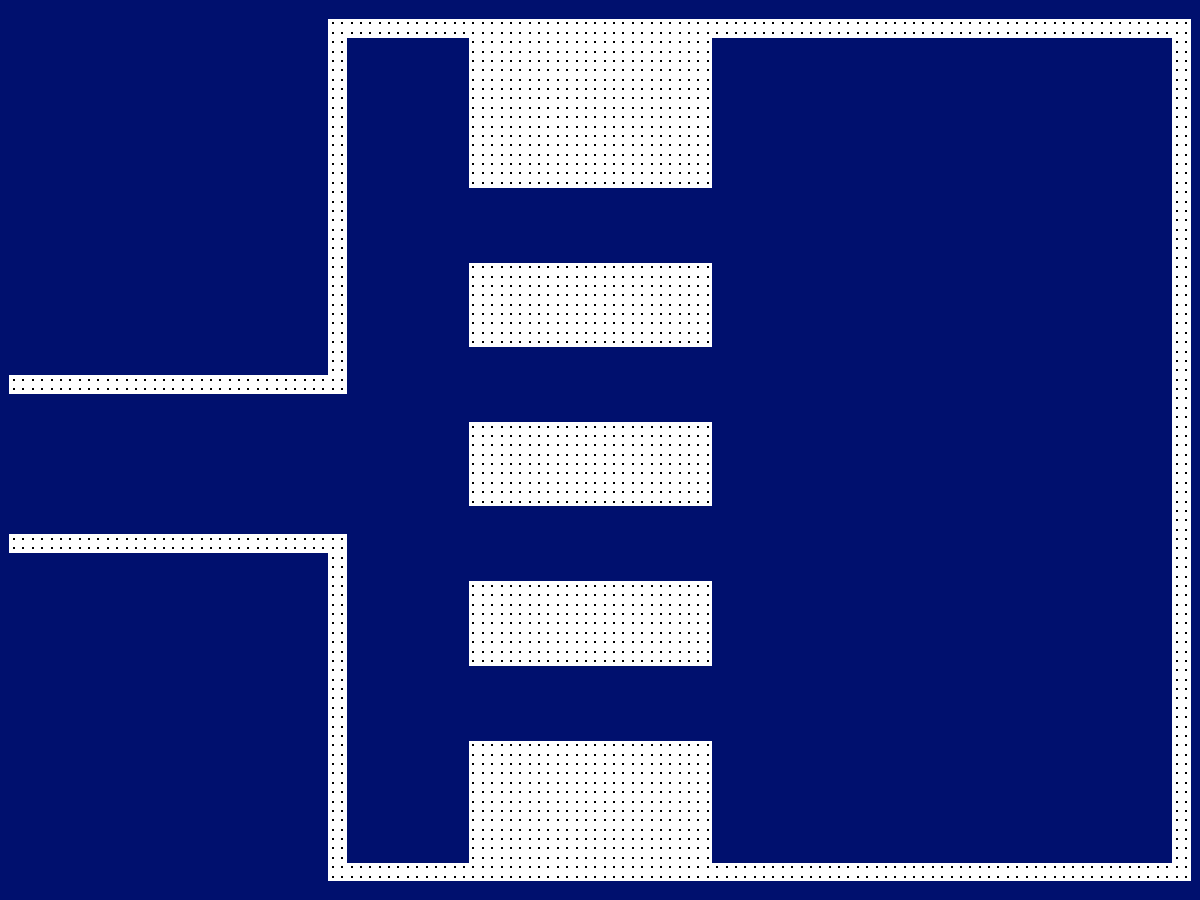
\includegraphics[width=\columnwidth]{../images/experiment_result_archive/scene.png}
\caption{Four-channel scenic-platform simulation scenario used in the numerical experiments.}
\label{fig:experiment_scene}
\end{figure}

\subsection{Mechanism Validation}
\label{sec:mechanism}

We first verify whether the two local modeling components have the intended behavioral meanings.
The fixed anisotropic mobility tensor $M(x;\eta_0)$ should reshape the channel attraction domain and induce entrance pre-alignment, whereas the admissible direction set $U(x;s)$ should remove prohibited directions and reroute flow through feasible channels.
When $M$ is applied to the middle channel, its flow share increases from $48.78\%$ in the baseline to $100.00\%$.
When a one-way rule excludes the originally dominant middle-channel direction, the middle-channel share becomes zero and the flow is redistributed to the upper, lower-middle, and bottom channels with shares $19.25\%$, $68.76\%$, and $12.00\%$, respectively.
For the bidirectional validation case, we use two diagnostic quantities.
The reverse-direction mass time is
\[
\mathrm{RMT}=
\sum_n\sum_{i\in\Omega_c}
\rho_i^n
\mathbf 1\{\mathbf u_i^n\cdot\tau_c<0\}
\Delta x^2\Delta t,
\]
which measures the cumulative simulation mass-time moving against the prescribed channel direction.
The counterflow cell-time is
\[
\mathrm{CCT}=
\sum_n\sum_{i\in\Omega_c}
\mathbf 1\{\rho_{i,+}^n>0,\rho_{i,-}^n>0\}\Delta t,
\]
which counts the cumulative grid-cell-time during which opposite-direction subpopulations coexist in the same channel region.
In the baseline bidirectional inflow test, the westbound middle-channel share, RMT, and CCT are $73.18\%$, $415.75$ simulation mass-time units, and $1213.76$ grid-cell-time units, respectively.
After imposing the eastbound one-way rule, all three quantities are reduced to zero.

\begin{figure*}[!t]
\centering

\includegraphics[width=0.82\textwidth]{../../codes/results/g1_mechanism_reframed/g1_um_configuration_flow_comparison.png}
\caption{Spatial transferability of the combined $U+M$ mechanism. Moving the controlled channel induces corresponding migration of dominant flow channels, streamlines, and density hotspots.}
\label{fig:g1_um_configuration}
\end{figure*}

Fig.~\ref{fig:g1_um_configuration} further shows that the combined $U+M$ mechanism is spatially transferable.
Changing the guided channel from the upper to the lower channel moves the dominant flow channel and local density hotspot accordingly.
These results support using the Bellman--conservation-law simulator as the lower-level evaluator for subsequent strategy optimization.

\subsection{Directional-Control Response}
\label{sec:strategy}

We next examine whether the discrete direction configuration $s$ creates nontrivial system-level trade-offs.
The response experiment uses thirteen interpretable direction settings: an all-free baseline, four single-entry cases, four single-return cases, and four one-channel-closure cases.
The direction code is ordered as $[T,M,LM,B]$, where $E$, $W$, $F$, and $X$ denote eastbound entry, westbound return, bidirectional free channel, and closure.

\begin{figure*}[!t]
\centering
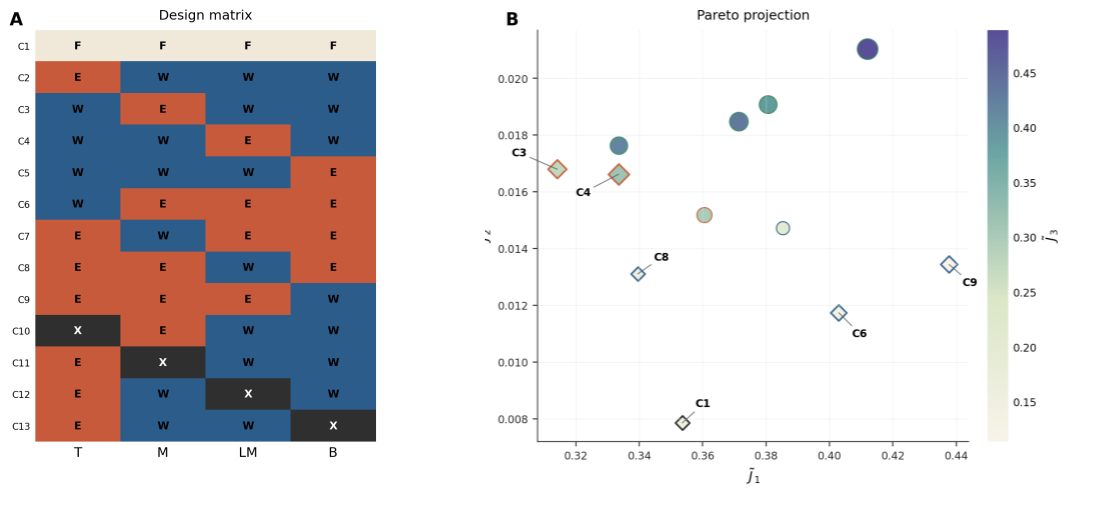
\includegraphics[width=0.92\textwidth]{../images/experiment_result_archive/g2_control_tradeoff_summary_ab.png}
\caption{Directional-control design matrix and objective-space trade-off. Color encodes $\tilde J_3$, marker size encodes the reduced dimensionless diagnostic objective $J^{(3)}$, and diamonds indicate non-dominated cases.}
\label{fig:g2_control_tradeoff}
\end{figure*}

Fig.~\ref{fig:g2_control_tradeoff} and Table~\ref{tab:g2_nondominated} show that no single direction configuration dominates all objectives.
This directional-response experiment summarizes the three reported terms by $J^{(3)}$; since no entrance-capacity curve is optimized, $\tilde J_4$ and $\tilde J_5$ are not used for ranking.
C8 (SR-LM, EEWE) obtains the lowest reduced objective $J^{(3)}=0.5102$, which is only $0.84\%$ lower than the all-free baseline C1.
C1 gives the lowest safety exposure $\tilde J_2=0.00785$, C3 gives the best efficiency term $\tilde J_1=0.3141$, and C9 gives the best load-balance term $\tilde J_3=0.1138$.
This non-monotonic response motivates automatic mixed-variable optimization rather than manual selection from a small set of rules.

\begin{table*}[!t]
\centering
\caption{Non-Dominated Directional-Control Cases}
\label{tab:g2_nondominated}
\scriptsize
\setlength{\tabcolsep}{4pt}
\begin{tabular}{c c c c c c c l}
\hline
Case & Policy & Code & $\tilde J_1$ & $\tilde J_2$ & $\tilde J_3$ & $J^{(3)}$ & Main characteristic \\
\hline
C1 & BSL & FFFF & 0.3535 & \textbf{0.00785} & 0.1531 & 0.5145 & Lowest exposure \\
C3 & SE-M & WEWW & \textbf{0.3141} & 0.01680 & 0.2741 & 0.6049 & Best efficiency but risk-concentrated \\
C4 & SE-LM & WWEW & 0.3335 & 0.01662 & 0.3131 & 0.6632 & Efficient but load-imbalanced \\
C6 & SR-T & WEEE & 0.4029 & 0.01174 & 0.1335 & 0.5482 & High return throughput \\
C8 & SR-LM & EEWE & 0.3395 & 0.01311 & 0.1576 & \textbf{0.5102} & Lowest reduced objective \\
C9 & SR-B & EEEW & 0.4377 & 0.01344 & \textbf{0.1138} & 0.5649 & Most balanced channel loads \\
\hline
\end{tabular}
\vspace{1mm}
\parbox{0.95\textwidth}{\scriptsize All objective terms in this table are dimensionless scaled normalized quantities. The reduced objective uses $\lambda_4=\lambda_5=0$ and is used only for directional-response diagnosis; it is not directly comparable with the full five-term objective in Table~\ref{tab:optimizer_summary}.}
\end{table*}

\subsection{Entrance-Rate Response}
\label{sec:entrance_rate_exp}

Direction rules alone cannot represent the case in which a channel remains open but its internal entrance must be metered.
We therefore fix $[T,M,LM,B]=[F,E,W,F]$ and scan four internal entrance-rate levels: no limit, high, medium, and low.
The rate upper bound acts on internal entrance crossing flow.
When attempted flow exceeds the upper bound, only the admitted flow crosses the interface, and the unreleased attempted flow remains upstream as waiting mass.
The entrance binding-time ratio is defined as the fraction of time steps in which attempted entrance flow exceeds the rate upper bound and creates unreleased attempted flow.
The unreleased attempted flow is
\[
U_{\mathrm{rel}}=
\int_0^T\sum_{c=1}^{C}
\left[
(A_c^+(t)-\hat A_c^+(t))_+
+
(A_c^-(t)-\hat A_c^-(t))_+
\right]dt,
\]
in simulation mass units, and its demand ratio is $r_{\mathrm{rel}}=U_{\mathrm{rel}}/\int_0^T\sum_c(A_c^+(t)+A_c^-(t))dt$.
This scan is a fixed-rate diagnostic experiment rather than a final optimizer-ranking experiment; the table therefore reports $J^{(3)}$, treats entrance waiting as a diagnostic quantity, and sets the smoothness contribution to zero because each policy uses a fixed rate level.

\begin{table*}[!t]
\centering
\caption{Response Under Internal Entrance-Rate Upper-Bound Levels}
\label{tab:entrance_rate_response}
\scriptsize
\setlength{\tabcolsep}{5pt}
\begin{tabular}{lrrrrrrr}
\hline
Level & $\tilde J_1$ & $\tilde J_2$ & $\tilde J_3$ & $J^{(3)}$ & $U_{\mathrm{rel}}$ & $r_{\mathrm{rel}}$ & Binding ratio \\
\hline
No limit & 0.6274 & 0.174 & 0.8838 & 1.6851 & 0.00 & 0 & 0.000 \\
High & 0.6262 & 0.358 & 0.8814 & 1.8652 & 241.40 & 70.8\% & 0.605 \\
Medium & 0.6228 & 0.443 & 0.8620 & 1.9276 & 329.26 & 82.6\% & 0.666 \\
Low & 0.6181 & 0.466 & 0.8493 & 1.9337 & 427.89 & 92.1\% & 0.721 \\
\hline
\end{tabular}
\vspace{1mm}
\parbox{0.95\textwidth}{\scriptsize $U_{\mathrm{rel}}$ is reported in simulation mass units. The safety column is a scaled normalized safety term, not a direct space-time percentage.}
\end{table*}

\begin{figure}[!t]
\centering
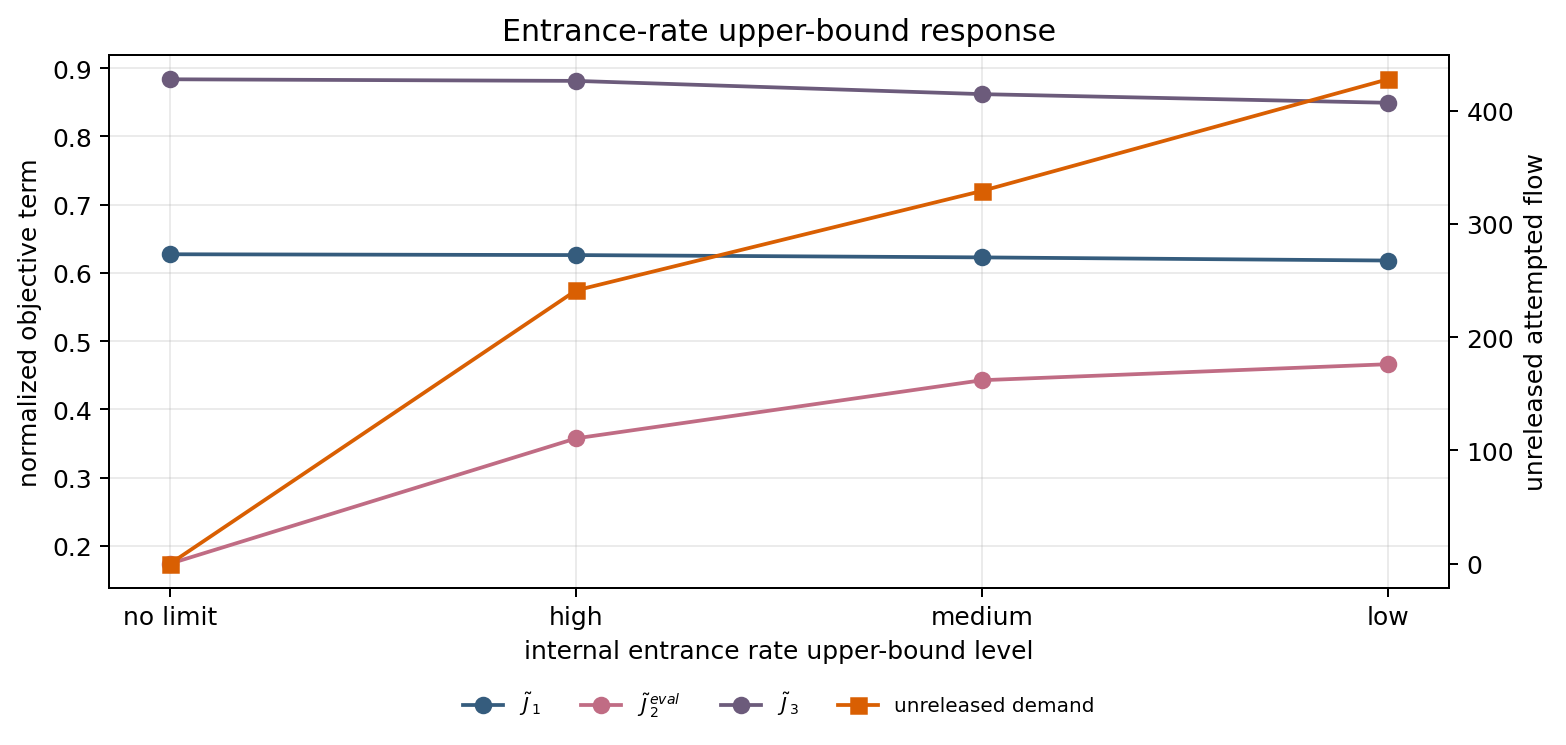
\includegraphics[width=\columnwidth]{../images/experiment_result_archive/g2/g2_capacity_levels.png}
\caption{Objective-term response under internal entrance-rate upper-bound levels. Tightening the upper bound changes safety exposure, load balance, and unreleased attempted flow; the latter is reported in simulation mass units.}
\label{fig:entrance_rate_response}
\end{figure}

Table~\ref{tab:entrance_rate_response} and Fig.~\ref{fig:entrance_rate_response} show that tightening the rate upper bound does not simply improve safety.
From the no-limit case to the low level, unreleased attempted flow increases from $0$ to $427.89$ simulation mass units, corresponding to $r_{\mathrm{rel}}=92.1\%$ of attempted entrance demand.
The binding ratio increases from $0$ to $0.721$, and the scaled normalized safety term $\tilde J_2$ increases from $0.174$ to $0.466$.
Thus, $q$ is a genuine continuous control variable that changes system response and must be optimized jointly with $s$.

\subsection{Horizontal Optimization Comparison}
\label{sec:optimal}

The horizontal comparison evaluates Prior Baseline, Random Search, Pure Simulated Annealing, Enumeration plus Differential Evolution, TPE-Mixed BO, and HCMBO.
All optimizers use $B=400$ candidate evaluations and top-$10$ high-fidelity rechecks over seeds $11$, $23$, $37$, $51$, and $73$.
The final HCMBO data are taken from the G7-D mainline, whereas the other baselines are taken from the G6 horizontal comparison under the same high-fidelity protocol.

\begin{table*}[!t]
\centering
\caption{High-Fidelity Performance Under the Full Five-Term Dimensionless Objective}
\label{tab:optimizer_summary}
\scriptsize
\setlength{\tabcolsep}{4pt}
\begin{tabular}{lrrrrrr}
\hline
Method & Mean objective & Std. & Median & Best & Worst & Feasible rate \\
\hline
HCMBO & \textbf{2.6338} & 0.3106 & \textbf{2.5065} & \textbf{2.4495} & 3.1851 & \textbf{100\%} \\
TPE-Mixed BO & 2.7403 & 0.2475 & 2.6288 & 2.5180 & 3.1345 & 80\% \\
Pure SA & 2.9248 & 0.1386 & 2.9203 & 2.7468 & 3.1049 & 60\% \\
Random Search & 3.0112 & 0.1319 & 2.9797 & 2.8821 & 3.2287 & 40\% \\
Enum-DE & 3.0597 & 0.1932 & 3.1004 & 2.7329 & 3.2500 & 40\% \\
Prior Baseline & 5.4774 & 0.0000 & 5.4774 & 5.4774 & 5.4774 & 0\% \\
\hline
\end{tabular}
\vspace{1mm}
\parbox{0.95\textwidth}{\scriptsize The reported objective is the full dimensionless scalar objective $J=\sum_{k=1}^{5}\lambda_k\tilde J_k$ after unified high-fidelity rechecking. These values are not directly comparable with the reduced diagnostic objective $J^{(3)}$ in Tables~\ref{tab:g2_nondominated}, \ref{tab:entrance_rate_response}, and \ref{tab:bund_transfer_metrics}.}
\end{table*}

Table~\ref{tab:optimizer_summary} shows that HCMBO achieves the lowest mean objective, lowest median objective, lowest best objective, and highest feasible rate.
In relative terms, the mean objective of HCMBO is $3.9\%$ lower than that of TPE-Mixed BO, since $(2.7403-2.6338)/2.7403=3.9\%$.
Because this is a normalized scalar objective, the percentage reduction should be interpreted as an improvement in the fixed-weight management score, rather than as a direct reduction in travel time or density exposure alone.
Relative to TPE-Mixed BO, HCMBO is better in $4/5$ paired seeds, with an average objective difference of $-0.1066$.
It also outperforms Random Search in all five seeds and outperforms Pure SA and Enum-DE in four of five seeds.
The remaining high objective in one HCMBO seed is mainly driven by a larger safety exposure term, indicating a residual need for stronger safety-constraint awareness.

\begin{figure}[!t]
\centering
\includegraphics[width=\columnwidth]{../../codes/results/final_hcmbo_cross_experiment_summary/final_method_best_objective.png}
\caption{Best high-fidelity full objective $J$ across seeds. The objective is dimensionless and lower is better. Range bars show the seed-wise spread, and the short vertical mark indicates the median.}
\label{fig:optimizer_best_objective}
\end{figure}

\begin{figure}[!t]
\centering
\includegraphics[width=\columnwidth]{../../codes/results/final_hcmbo_cross_experiment_summary/final_method_convergence.png}
\caption{Best-so-far convergence curves under the same $400$-evaluation budget. The inset highlights the final-stage separation among methods.}
\label{fig:optimizer_convergence}
\end{figure}

\begin{figure}[!t]
\centering
\includegraphics[width=\columnwidth]{../../codes/results/final_hcmbo_cross_experiment_summary/final_method_control_profiles.png}
\caption{Best-solution entrance-rate profiles for Random Search, Pure SA, Enum-DE, TPE-Mixed BO, and HCMBO. The common direction structure is $[T,M,LM,B]=[W,E,E,W]$ for several methods, but the segment-wise rate allocations differ substantially.}
\label{fig:control_profiles}
\end{figure}

Figs.~\ref{fig:optimizer_best_objective}--\ref{fig:control_profiles} provide complementary visual evidence.
TPE-Mixed BO descends quickly in the early evaluations, but HCMBO continues to improve in the middle and late stages and reaches the lowest final region.
The entrance-rate profiles show that performance differences are not only caused by choosing a discrete direction code; they also arise from detailed segment-wise rate allocation within the same direction structure.

\subsection{HCMBO Ablation}
\label{sec:ablation}

The ablation experiments examine whether the control variables and search mechanisms used by HCMBO are necessary.
First, direction and entrance-rate variables must be optimized jointly.
Optimizing only direction with a fixed high rate gives best high-fidelity objective $3.3751$, while optimizing only rates under prior directions gives $3.3140$; both are clearly worse than joint optimization.
Second, short-horizon low-fidelity hard screening increases the best objective to $2.9441$ and yields an infeasible best candidate, because early simulations do not reliably reflect long-horizon entrance waiting and load redistribution.
Third, removing the entrance-waiting penalty slightly reduces the scalar objective to $2.6015$, but increases unreleased attempted flow to approximately $3.24\times10^3$ simulation mass units, showing that waiting should remain in the management objective.

\begin{table*}[!t]
\centering
\caption{Search-Mechanism Ablation Under Seed 23}
\label{tab:search_ablation}
\scriptsize
\setlength{\tabcolsep}{4pt}
\begin{tabular}{lrrrrl}
\hline
Variant & Best objective & Feasible rate & $\tilde J_2$ & Unreleased flow (sim. mass) & Main meaning \\
\hline
HCMBO & \textbf{2.4495} & 100\% & \textbf{1.6759} & $2.55{\times}10^3$ & Structured direction-wise rate search \\
Queue-aware LCB & 2.6162 & 100\% & 1.8521 & $\mathbf{2.41{\times}10^3}$ & Queue-aware acquisition \\
RF-style constrained BO & 2.6162 & 100\% & 1.8521 & $\mathbf{2.41{\times}10^3}$ & Constraint surrogate variant \\
Adaptive racing & 2.6561 & 100\% & 1.9474 & $3.20{\times}10^3$ & Stage-wise budget concentration \\
Adaptive racing + queue-aware & 2.6683 & 100\% & 1.7862 & $2.66{\times}10^3$ & Combined racing and queue signal \\
Trust-region search & 3.0317 & 100\% & 1.9224 & $3.97{\times}10^3$ & Local trust-region search \\
\hline
\end{tabular}
\vspace{1mm}
\parbox{0.95\textwidth}{\scriptsize Unreleased flow is unreleased attempted entrance flow in simulation mass units.}
\end{table*}

Table~\ref{tab:search_ablation} shows that the final HCMBO mainline obtains the lowest scalar objective among the tested variants.
Queue-aware LCB and RF-style constrained BO reduce unreleased attempted flow to approximately $2.41\times10^3$ simulation mass units, but their scalar objective increases to $2.6162$.
Thus, queue information is useful for executable and safety-aware extensions, whereas the final mainline should retain structured direction-wise rate search as the primary budget allocation mechanism.

\subsection{Transfer Validation on a Bund-Inspired Scenario}
\label{sec:bund_transfer}

The preceding experiments use a standardized four-channel platform scenario to verify modeling mechanisms and optimization behavior under controlled conditions.
As a supplementary validation, we further construct a simplified abstract scenario inspired by the spatial form of the Shanghai Bund waterfront.
This experiment does not claim to reproduce all architectural details of the real site.
Instead, it preserves the Bund sightseeing platform, the lateral passage connections, the major inflow location, and the dominant movement direction, so as to examine whether an HCMBO-derived policy can still change the load distribution in a more realistic spatial outline.

\begin{figure*}[!t]
\centering
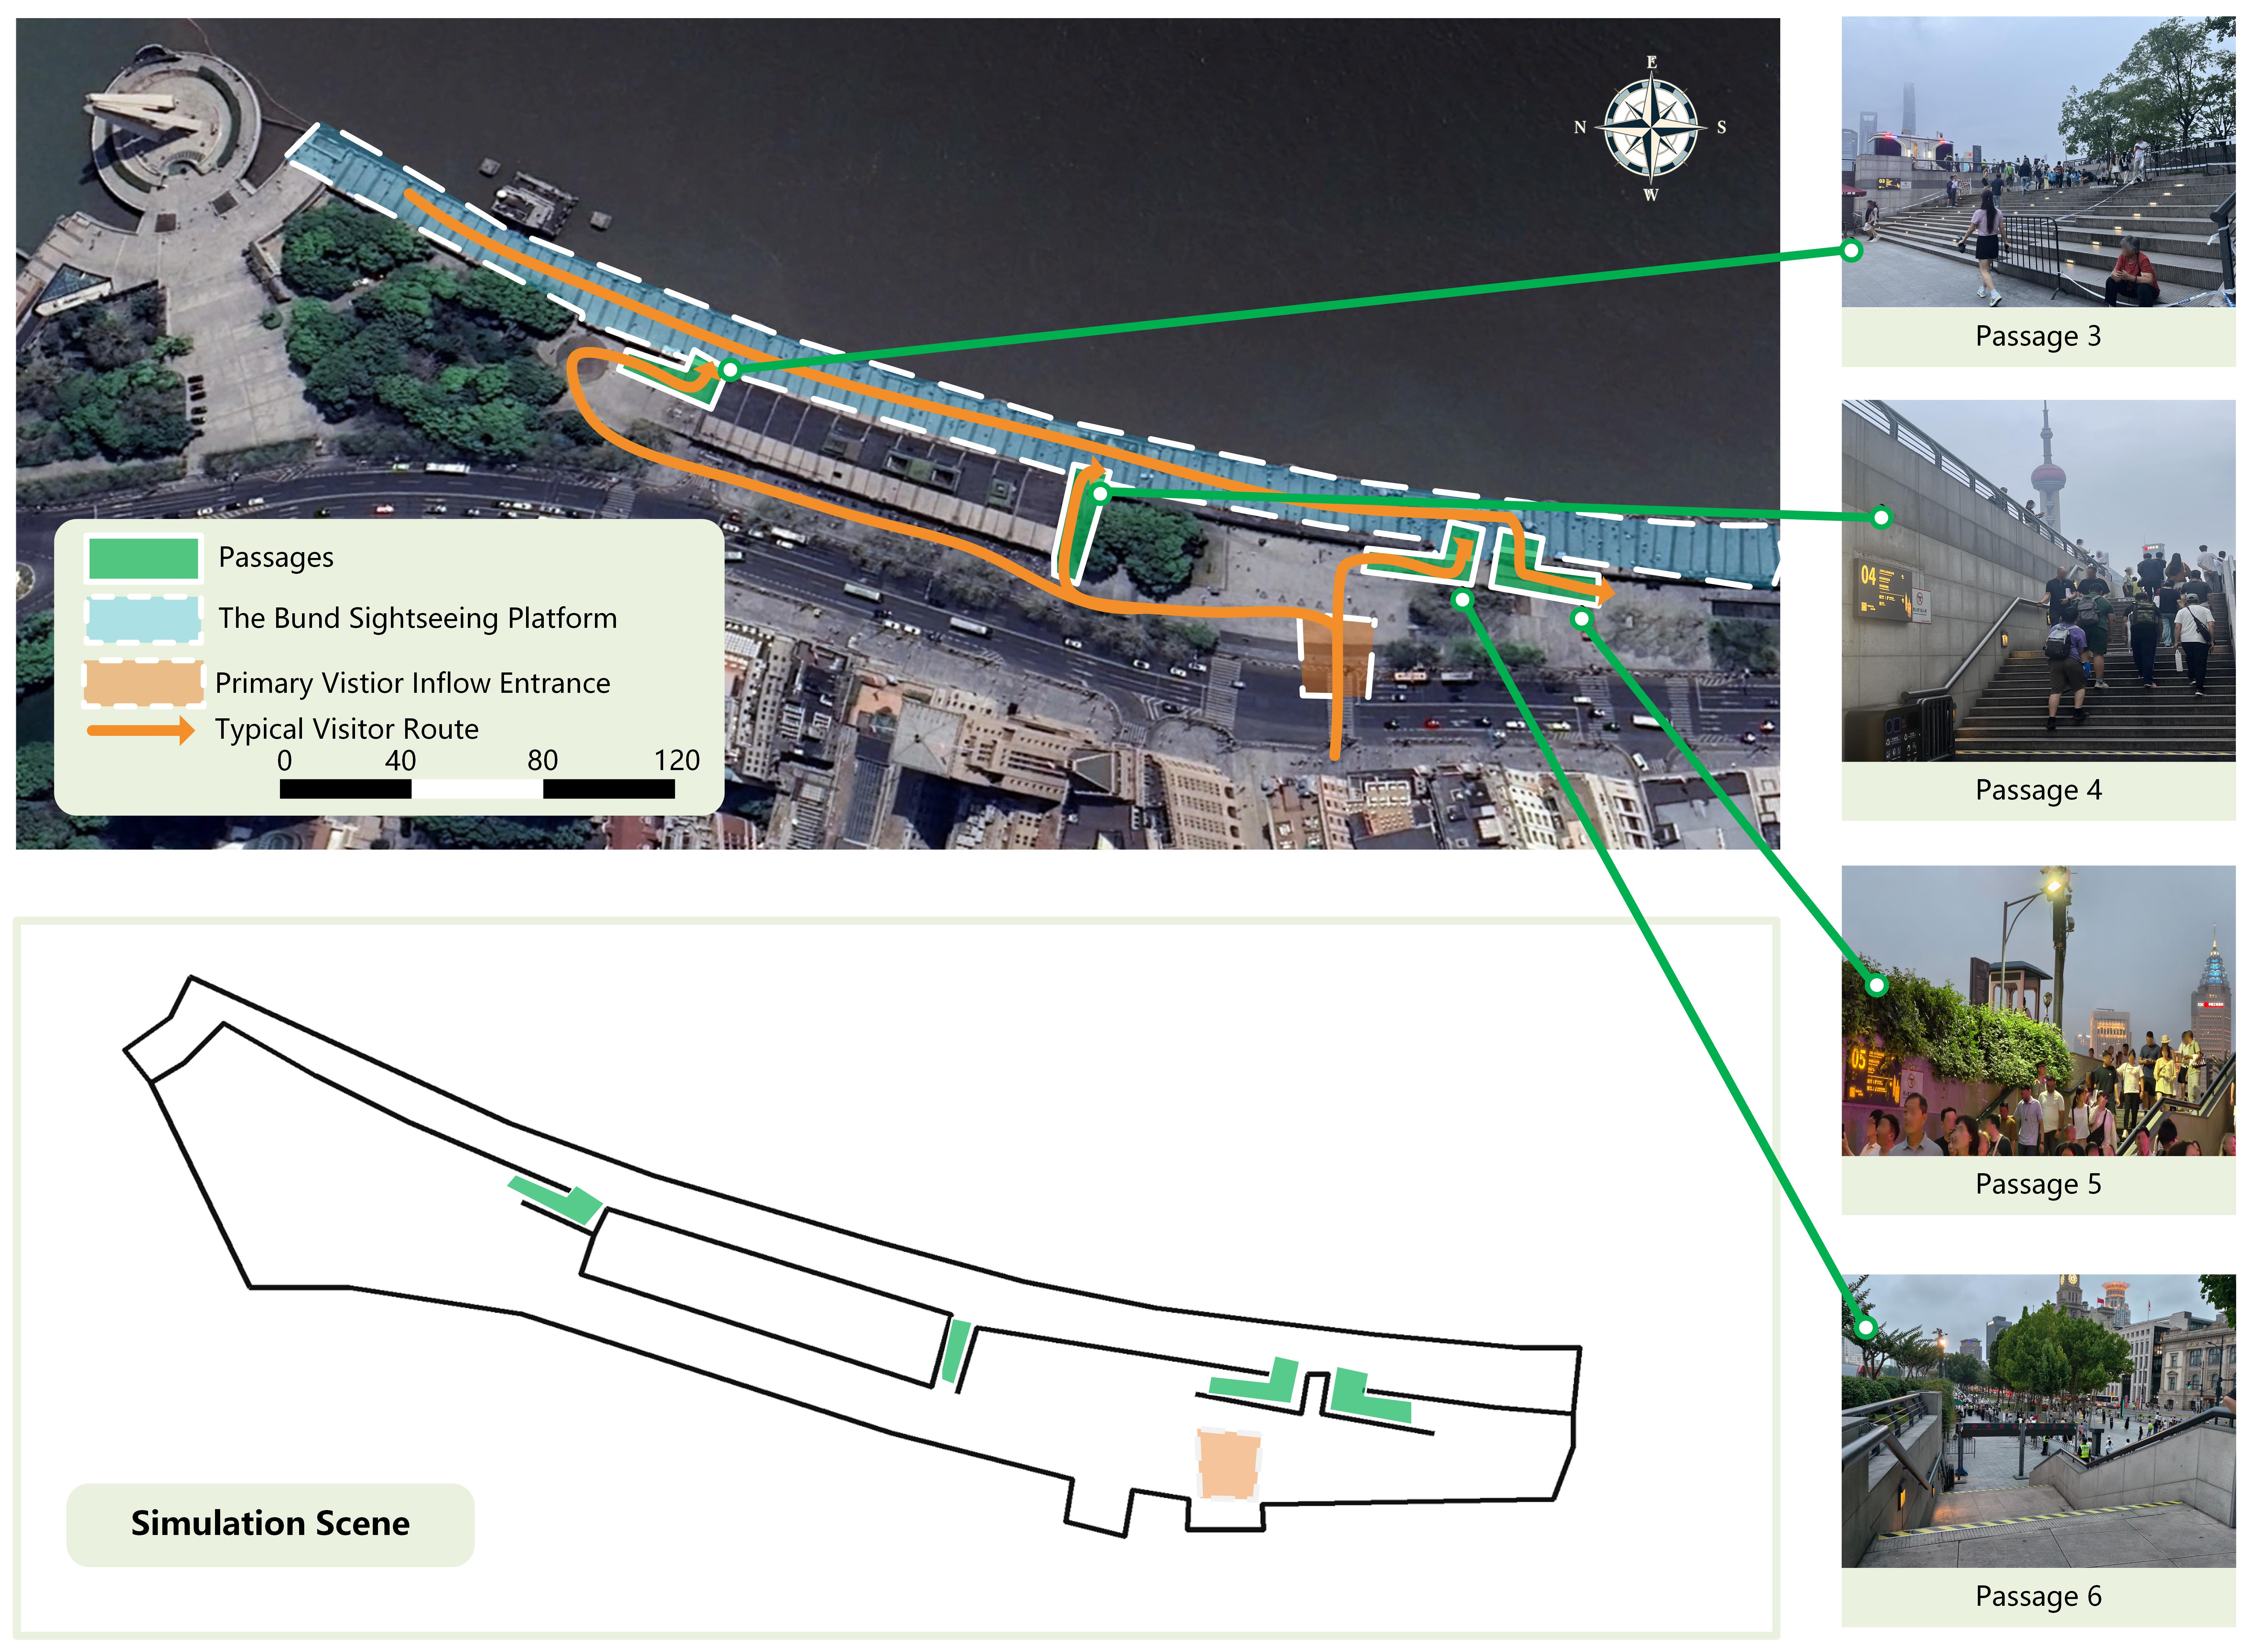
\includegraphics[width=0.82\textwidth]{../图表/visio架构图/外滩场景示意图_页-7.jpg}
\caption{Real Bund scene and its simplified simulation abstraction. The abstraction retains the Bund sightseeing platform boundary, the main entrance, and the passage connections used for control validation. The satellite basemap was obtained from Google Maps. The right-side local photographs were shot in the Shanghai Bund waterfront passage area by the Tongji Public Safety Experimental Team, June 21, 2026.}
\label{fig:bund_transfer_scene}
\end{figure*}

The computational grid has resolution $512\times224$ with $\Delta x=0.125$.
Pedestrians enter from the outer-side entrance, pass through the middle connecting channels, and move toward the Bund sightseeing platform and its central target region.
The inflow-rate multiplier is $3.0$, corresponding to an actual inflow rate of $0.24$; the maximum density is $\rho_{\max}=4.0$, and the transition smoothing parameter is $\kappa=32$.
The experimental channels \texttt{channel\_1}, \texttt{channel\_2}, \texttt{channel\_3}, and \texttt{channel\_4} correspond to the locally named Bund Passages 3, 4, 5, and 6, respectively.
Both the controlled and uncontrolled groups use $1600$ steps and a time horizon of $50$.
For the controlled group, the transferred entrance-rate bounds are multiplied by a capacity-scale factor of $3$, providing a less restrictive entrance-capacity setting.

The controlled group uses the best HCMBO policy obtained from the multi-direction high-fidelity recheck.
Its reduced high-fidelity objective in the optimization stage is $0.7350$, and its direction structure leaves the upper and lower channels bidirectional while assigning opposite dominant directions to the two middle channels.
Table~\ref{tab:bund_transfer_q} reports the effective two-segment entrance-rate upper bounds after applying the capacity-scale factor of $3$.
The rate upper bounds are measured in simulation mass per unit time.

\begin{table*}[!t]
\centering
\caption{Effective Entrance-Rate Upper Bounds in the Bund Transfer Experiment}
\label{tab:bund_transfer_q}
\scriptsize
\setlength{\tabcolsep}{5pt}
\begin{tabular}{l l l r r}
\hline
Experimental channel & Local passage name & Entrance side & Segment 1 & Segment 2 \\
\hline
\texttt{channel\_1} & Bund Passage 3 & Forward entrance & 0.2474 & 0.6000 \\
\texttt{channel\_1} & Bund Passage 3 & Reverse entrance & 0.2269 & 0.0000 \\
\texttt{channel\_2} & Bund Passage 4 & Forward entrance & 0.6000 & 0.1688 \\
\texttt{channel\_2} & Bund Passage 4 & Reverse entrance & 0.0000 & 0.0000 \\
\texttt{channel\_3} & Bund Passage 5 & Forward entrance & 0.0000 & 0.0000 \\
\texttt{channel\_3} & Bund Passage 5 & Reverse entrance & 0.2560 & 0.4975 \\
\texttt{channel\_4} & Bund Passage 6 & Forward entrance & 0.3785 & 0.2169 \\
\texttt{channel\_4} & Bund Passage 6 & Reverse entrance & 0.2215 & 0.2122 \\
\hline
\end{tabular}
\end{table*}

Table~\ref{tab:bund_transfer_metrics} compares the controlled and uncontrolled groups under the same high-fidelity protocol.
It separates dimensionless normalized terms from raw simulation diagnostics.
The reduced objective $J^{(3)}$ decreases from $1.0140$ to $0.7410$, corresponding to an absolute reduction of approximately $0.2730$ and a relative reduction of $26.9\%$.
The main improvement comes from the load-balance term $\tilde J_3$, which decreases by $51.9\%$, from $0.6043$ to $0.2908$.
In contrast, $\tilde J_1$ increases by $8.7\%$ and $\tilde J_2$ increases by $25.7\%$.
This indicates that the transferred policy changes how pedestrians use the channels, rather than merely reducing all density values uniformly.

\begin{table*}[!t]
\centering
\caption{Controlled and Uncontrolled Results in the Bund Transfer Experiment}
\label{tab:bund_transfer_metrics}
\scriptsize
\setlength{\tabcolsep}{4pt}
\begin{tabular}{l r r r}
\hline
Dimensionless term & Controlled & Uncontrolled & Relative change \\
\hline
$J^{(3)}$ & 0.7410 & 1.0140 & $-26.9\%$ \\
$\tilde J_1$ & 0.4145 & 0.3813 & $+8.7\%$ \\
$\tilde J_2$ & 0.0357 & 0.0284 & $+25.7\%$ \\
$\tilde J_3$ & 0.2908 & 0.6043 & $-51.9\%$ \\
\hline
\end{tabular}

\vspace{1.5mm}
\begin{tabular}{l r r l}
\hline
Raw diagnostic & Controlled & Uncontrolled & Unit \\
\hline
Final cumulative sink flow & 6.82 & 8.57 & sim. mass \\
Final cumulative inflow & 11.92 & 12.00 & sim. mass \\
Final system mass & 7.85 & 6.18 & sim. mass \\
Peak density maximum & $\approx 4.0$ & $\approx 4.0$ & sim. mass/area \\
Average mean density & $3.47{\times}10^{-3}$ & $3.21{\times}10^{-3}$ & sim. mass/area \\
Attempted entrance flow & 7.65 & 0 & sim. mass \\
Actual entrance flow & 5.78 & 0 & sim. mass \\
Unreleased attempted flow & 1.87 & 0 & sim. mass \\
\hline
\end{tabular}
\end{table*}

The channel-flow shares in Table~\ref{tab:bund_transfer_flux} further explain this reduction.
In the uncontrolled group, $82.30\%$ of the channel flow concentrates on \texttt{channel\_4}, i.e., Bund Passage 6.
After applying the HCMBO policy, the flow is redistributed mainly to \texttt{channel\_2} and \texttt{channel\_3}, whose combined share reaches approximately $91.34\%$.

\begin{table}[!t]
\centering
\caption{Channel-Flow Shares in the Bund Transfer Experiment}
\label{tab:bund_transfer_flux}
\scriptsize
\setlength{\tabcolsep}{4pt}
\begin{tabular}{l l r r}
\hline
Channel & Local name & Controlled & Uncontrolled \\
\hline
\texttt{channel\_1} & Bund Passage 3 & 2.83\% & 0.32\% \\
\texttt{channel\_2} & Bund Passage 4 & 30.38\% & 1.35\% \\
\texttt{channel\_3} & Bund Passage 5 & 60.96\% & 16.03\% \\
\texttt{channel\_4} & Bund Passage 6 & 5.83\% & 82.30\% \\
\hline
\end{tabular}
\vspace{1mm}
\parbox{\columnwidth}{\scriptsize Channel-flow shares are computed as $R_c(T)/\sum_{j=1}^{C}R_j(T)$, where $R_c(T)$ is the realized cumulative admitted throughput of channel $c$ during the simulation horizon.}
\end{table}

\begin{figure*}[!t]
\centering
\includegraphics[width=0.95\textwidth]{../../codes/results/bund_control_comparison_hcmbo_capacity3/figures/bund_comparison_density_panel_steps_0050_0350_0900_1500.png}
\caption{Density evolution comparison between uncontrolled and controlled cases at steps 50, 350, 900, and 1500. The controlled policy redistributes the later-stage flow from the terminal channel toward the middle-channel group.}
\label{fig:bund_transfer_density_panel}
\end{figure*}

Fig.~\ref{fig:bund_transfer_density_panel} visualizes the density evolution at steps $50$, $350$, $900$, and $1500$.
Both groups initially form a local density concentration near the right-side target region of the Bund sightseeing platform, reflecting the same inflow and target-attraction structure.
At later stages, the uncontrolled case remains more concentrated around the terminal channel and the adjacent Bund sightseeing platform area, whereas the controlled case develops a more stable flow band through the middle-channel group.
This visual evidence is consistent with the channel-share statistics and confirms that the main effect of the HCMBO policy is load redistribution across channels.

The supplementary transfer experiment also reveals an important trade-off.
Compared with the uncontrolled group, the controlled group shows a higher efficiency term ($\tilde J_1$ increases from $0.3813$ to $0.4145$) and a slightly higher safety-exposure term ($\tilde J_2$ increases from $0.0284$ to $0.0357$).
At the same time, its cumulative sink flow is smaller ($6.82$ versus $8.57$ simulation mass units) and its final system mass is larger ($7.85$ versus $6.18$).
Therefore, the transferred HCMBO policy should not be interpreted as uniformly improving safety and efficiency.
Rather, under the present reduced-objective weights, it reduces $J^{(3)}$ mainly by improving channel-load balance, while sacrificing part of the exit throughput and travel efficiency.
The capacity-scale factor of $3$ reduces unreleased attempted flow to $1.87$ simulation mass units, but it does not remove the efficiency cost of the control policy.
Overall, the supplementary Bund-inspired experiment shows that the optimized HCMBO policy can still reduce the reduced objective and redistribute flow away from the dominant terminal channel in a simplified real-world spatial abstraction.
However, the improvement is accompanied by unreleased attempted entrance flow, lower exit throughput, and higher residual mass in the system.
Future deployment-oriented extensions should therefore include explicit throughput constraints, waiting upper bounds, or multi-weight scenario analysis to avoid obtaining policies that improve load balance at the cost of overly strong metering.



\section{Conclusion}
\label{sec:conclusion}

We proposed a macroscopic crowd management framework for open pedestrian zones that jointly models passage-direction rules, geometric guidance, multi-stage route behavior, and internal entrance-rate control.
The framework links an interpretable crowd-flow simulator with HCMBO, so that direction settings and entrance-rate profiles can be optimized together under a limited simulation budget.

The experiments show that the model components produce the intended behavioral effects and that the two control dimensions are not interchangeable.
Direction settings create non-monotonic trade-offs among efficiency, safety exposure, and load balance, while entrance-rate limits change unreleased attempted flow, binding-time ratios, and local risk patterns.
Under five random seeds and unified high-fidelity rechecking, HCMBO obtains the lowest mean full management objective among the tested baselines.
It reduces the fixed-weight score by 3.9 percent relative to TPE-Mixed BO and maintains a 100 percent feasible rate.
Ablation results indicate that joint direction--rate optimization, avoiding short-horizon hard screening, and using structured direction-wise rate search are central to this performance.

The Bund-inspired transfer experiment further shows that an HCMBO-derived policy can still alter flow organization in a simplified real-world spatial abstraction.
In that experiment, the reduced objective decreases by 26.9 percent.
This reduction mainly occurs because the policy redistributes flow away from the dominant terminal channel and improves load balance across the middle-channel group.
However, this gain is accompanied by higher residual system mass, lower exit throughput, and unreleased attempted entrance flow.
Therefore, the transfer result should be interpreted as evidence of mechanistic transferability and load-redistribution capability, not as a ready-to-deploy operational plan for the Bund area.

The current study still has limitations.
The experiments are based on simplified geometries, fixed objective weights, and finite random seeds; one HCMBO seed still exhibits relatively high safety exposure; and real crowd calibration, online demand updates, and executable field constraints are not yet included.
Future work will extend the framework to richer real geometries, broader demand and seed settings, stronger constraint-aware optimization baselines, multi-weight Pareto analysis, and calibration against field observations.

\balance

\bibliographystyle{IEEEtran}
\bibliography{references}

\end{document}
